%%%%%%%%%%%%%%%%%%%%%%%%%%%%%%%%%%%%%%%%%%%%%%%%%%%%%%%%%%%%%%%%%%%%%%%%%%%
%
%  sections.tex
%
%  Content for Ludwig documentation.
%
%  $Id$
%
%  Edinburgh Soft Matter and Statistical Physics Group and
%  Edinburgh Parallel Computing Centre
%
%  Kevin Stratford (kevin@epcc.ed.ac.uk)
%  (c) 2008 The University of Edinburgh
%
%%%%%%%%%%%%%%%%%%%%%%%%%%%%%%%%%%%%%%%%%%%%%%%%%%%%%%%%%%%%%%%%%%%%%%%%%%%


\section{The Lattice Boltzmann Method}

We review here the lattice Boltzmann method applied to single
phase problems.

\subsection{The Navier Stokes Equation}

We seek to solve the isothermal Navier-Stokes equations which, often
written in vector form, express mass conservation
\begin{equation}
\partial_t \rho + \boldsymbol{\nabla}.(\rho\mathbf{u}) = 0
\label{eq_mass1}
\end{equation}
and the conservation of momentum
\begin{equation}
\partial_t (\rho\mathbf{u}) + \boldsymbol{\nabla}.(\mathbf{\rho uu}) =
-\boldsymbol{\nabla}p + \eta \nabla^2 \mathbf{u}
+\zeta \boldsymbol{\nabla}(\boldsymbol{\nabla}.\mathbf{u}).
\label{eq_momentum1}
\end{equation}
Equation~\ref{eq_mass1} expresses the local rate of change of the
density $\rho(\mathbf{r}; t)$ as the divergence of the flux of
mass associated with the velocity field $\mathbf{u}(\mathbf{r}; t)$.
Equation~\ref{eq_momentum1} expresses Newton's second law for
momentum, where the terms on the right hand side represent the
force on the fluid.

For this work, it is more convenient to rewrite these equations
in tensor notation, where Cartesian coordinates ${x,y,z}$ are
represented by indices $\alpha$ and $\beta$, viz
\begin{equation}
\partial_t \rho + \nabla_\alpha (\rho u_\alpha) = 0
\end{equation}
and
\begin{equation}
\partial_t (\rho u_\alpha) + \nabla_\beta (\rho u_\alpha u_\beta)
= -\nabla_\alpha p
+  \eta \nabla_\beta (u_\alpha \nabla_\beta + \nabla_\alpha u_\beta)
+ \zeta \nabla_\alpha (\nabla_\gamma u_\gamma).
\end{equation}
Here, repeated indices are understood to be summed over.
The conservation law is seem better if the forcing terms of the
right hand side are combined in the fluid stress $\Pi_{\alpha\beta}$
so that
\begin{equation}
\partial_t (\rho u_\alpha) +\nabla_\beta \Pi_{\alpha\beta} = 0.
\end{equation}
In this case the expanded expression for the stress tensor is
\begin{equation}
\Pi_{\alpha\beta} = p \delta_{\alpha\beta} + \rho u_\alpha u_\beta 
+ \eta \nabla_\alpha v_\beta + \zeta (\nabla_\gamma v_\gamma)\delta_{\alpha\beta}
\end{equation}
where $\delta_{\alpha\beta}$ is that of Kroneker. Th Navier-Stokes
equations have 10 degrees of freedom (or hydrodynamic modes) being
$\rho$, three components of the mass flux $\rho u_\alpha$, and 6 independent
modes from the (symmetric) stress tensor $\Pi_{\alpha\beta}$.


\subsection{The Distribution Function and its Moments}

In lattice Boltzmann, the density and velocity of the continuum fluid
are replaced by their discrete counterparrts, the distribution function
$f_i(\mathbf{r}; t)$ and the discrete velocity space $c_{i\alpha}$.
It is possible to relate the hydrodynamic modes to distribution
function via its moments, so
\begin{equation}
\rho = \sum_i f_i,  \,
\rho u_\alpha = \sum_i f_i c_{i\alpha},  \,
\Pi_{\alpha\beta} = \sum_i f_i c_{i\alpha} c_{i\beta.}
\end{equation}
here, the index of the summation is over the number of discrete
velocities used $n$, which in three dimensions is generally
denoted by D3Q$n$. We restrict our discussion to D3Q15 and
D3Q19 (see below).

In general, the number of modes supported in $n$ and these can
be written as
\begin{equation}
M^a(\mathbf{r};t) = \sum_i m_i^a f_i(\mathbf{r};t),
\end{equation}
where $m_i^a$ is the corresponding eigenvector of the collision
maxtrix (see section blah). For example, if $m_i^a = 1$ then the
mode $M^a$ is the density. Correspondingly, the distribution
function can be related to the modes $M^a$ via
\begin{equation}
f_i() = \sum_a w_i m_i^a M^a() N^a
\end{equation}

\subsubsection{Hydrodynamic modes}

\subsubsection{D3Q15 ghost modes}

\subsubsection{D3Q19 ghost modes}

\subsection{The Lattice Boltzmann Equation}

\subsection{The Collision}

\subsection{External Body Forces}

\subsection{Fluctuating LBE}

It is possible \cite{adhikari2005} to simulate fluctuating
hydrodynamics for an isothermal fluid via the inclusion of
a fluctuating stress $\sigma_{\alpha\beta}$:
\begin{equation}
\Pi_{\alpha\beta} = p\delta_{\alpha\beta} + \rho u_\alpha u_\beta
+ \eta_{\alpha\beta\gamma\delta} \nabla_\gamma u_\delta + \sigma_{\alpha\beta}.
\end{equation}
The fluctuation-dissipation theorem relates the magnitude of this
random stress to the isothermal temperature and the viscosity.

In the LBE, this translates to the addition of a random contribution
$\xi_i$ to the distribution at the collision stage, so that
\begin{equation}
\ldots + \xi_i.
\end{equation}

For the conserved modes $\xi_i = 0$. For all the non-conserved modes,
i.e., those with dissipation, the fluctuating part may be written
\begin{equation}
\xi_i (\mathbf{r}; t) = w_i m_i^a \hat{\xi}^a (\mathbf{r}; t) N^a
\end{equation}
where $\hat{\xi}^a$ is a noise termwhich has a variance determined
by the relaxation time for given mode
\begin{equation}
\left< \hat{\xi}^a \hat{\xi}^b \right> =
\frac{\tau_a + \tau_b + 1}{\tau_a \tau_b}
\left< \delta M^a \delta M^b \right>.
\label{eq_fvar}
\end{equation}

\subsubsection{Fluctuating stress}

For the stress, the random contribution to the distributions is
\begin{equation}
\xi_i = w_i \frac{Q_{i\alpha\beta} \hat{\sigma}_{\alpha\beta}}{4c_s^2}
\end{equation}
where $\hat{\sigma}_{\alpha\beta}$ is a symmtric matrix of random
variates drawn from a Gaussian distribution with variance given
by equation~\ref{eq_fvar}. In the case that the shear and bulk
viscosities are the same, i.e., there is a single relaxation
time, then the variances of the six independent components of
the matrix are given by
\begin{equation}
\left< \hat{\sigma}_{\alpha\beta} \hat{\sigma}_{\mu\nu} \right> =
\frac{2\tau + 1}{\tau^2}
(\delta_{\alpha\mu}\delta_{\beta\nu} + \delta_{\alpha\nu} \delta_{\beta\mu}).
\end{equation}


\subsubsection{Fluctuating ghost modes: D3Q15}

\subsubsection{Fluctuating ghost modes: D3Q19}



\subsection{The Propagation}



\subsection{Solid bodies and Bounce-Back on Links}

A very general method for the representation of solid objects
within the LB approach was put forward by Ladd \cite{l94a, l94b}.
Solid objects (of any shape) are defined by a boundary surface
which intersects some of the velocity vectors $\mathbf{c}_i$
joining lattice nodes. Sites inside are designated solid, while
sites outside remain fluid. The correct boundary condition is
defined by identifying \textit{links} between fluid and solid
sites, which allows those elements of the distribution which would
cross the boundary at the propagation step to be ``bounced-back''
into the fluid. This bounce-back on links is an efficient method
to obtain the  correct hydrodynamic interaction between solid
and fluid.

\subsubsection{Boundary walls}

\subsection{Colloids}

\subsubsection{General}

Colloidal particles are assumed to be spherical with a geometrical
centre $\mathbf{r}_c$, which is also the centre of mass. The
centre is allowed to move continuously across the lattice
with velocity $\mathbf{U}$; the particle has an angular velocity
$\mathbf{\Omega}$. The surface of the colloid is defined by an
input radius, $a_0$, which determines which lattice nodes are
inside or outside the colloid. (The hydrodynamic properties of
the colloid are specified by a different radius $a_h$ --- more
of this later.) The boundary links are then the set of vectors
joining lattice nodes which intersect the spherical surface
$\{\mathbf{c}_b\}$. A schematic picture is presented in
Figure~\ref{fig_coll2}. Note that a lattice node exactly at
the solid-fluid interface is defined to be outside the colloid.

In the original approach of Ladd, fluid occupied nodes both inside
and outside the particle. The effect of the ``internal fluid'' is
known to be restricted to short time scales (compared to the
characteristic time $a_0^2/\nu$), on which the fluid inside the
particle relaxes to a solid body rotation \cite{heemels}. There
are a number of problems related to the internal fluid, so we
use fully solid particles.

Nguyen and Ladd.

For each boundary link, it is useful to define a boundary vector,
$\mathbf{r}_b$, which connects the centre of the colloid to the
appropriate boundary node (note that the length of this vector is
not necessarily equal to the input radius of the colloid).


\begin{figure}[tb]
\begin{center}
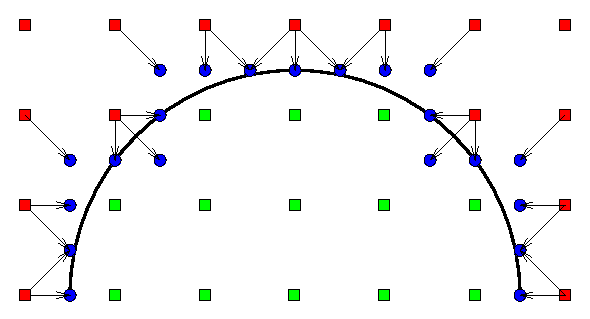
\includegraphics{xfig/colloidhalflinksnew.eps}
\end{center}
\caption{Boundary links for a colloidal particle in two dimensions
with D2Q9 (half the particle is shown). Links join fluid sites (red)
to solid sites (green) and
intersect the circular shell radius $a_0$. Boundary nodes (circles)
lie exactly half way between pairs of lattice nodes. The generalisation
to three dimensions is straightforward.}
\label{fig_coll2}
\end{figure}

A \textit{boundary node} halfway between fluid nodes which are joined
by a boundary link. The position of the boundary node is always
exactly halfway along the boundary link ($\mathbf{r} + \frac{1}{2}\mathbf{c}_b
\Delta t$) regardless of the actual position of the intersection
of the colloid surface and the boundary link.
The colloid therefore has a discrete representation which becomes a
better approximation to the sphere as the input radius becomes larger;
this approximation is known to be reasonably good for $a_0 > 5\Delta x$.



\subsubsection{Bounce-back on links}

The standard boundary condition required for the solid-fluid
interface of a moving particle is described by Ladd \cite{l94b},
and is generally refered to as bounce-back on links (BBL).
A boundary link is defined as joining a node $\mathbf{r}$
inside the particle to one outside at $\mathbf{r} + \mathbf{c}_b \Delta t$.
If the post-collision distributions are denoted by $f^\ast$, then
the distributions must be reflected at the solid surface so that
\begin{equation}
\label{eq:bbl1}
f_{b'}(\mathbf{r}; t + \Delta t) = f_b^\ast (\mathbf{r}; t)
- \frac{2w_{c_b} \rho \mathbf{u}_b.\mathbf{c}_b}{c_s^2}
\end{equation}
where the boundary link $\mathbf{c}_{b'} = -\mathbf{c}_b$. The velocity
at the boundary
\begin{equation}
\label{eq:ub}
\mathbf{u}_b = \mathbf{U} + \mathbf{\Omega}\times\mathbf{r}_b
\end{equation}
is determined by the particle linear velocity $\mathbf{U}$ and angular
velocity $\mathbf{\Omega}$. The change in momentum described by

The force exerted on a
single link is
\begin{equation}
\mathbf{F}_b(\mathbf{r} + {\scriptstyle\frac{1}{2}}\mathbf{c}_b\Delta t;
t + {\scriptstyle\frac{1}{2}}\Delta t) = \frac{\Delta x^3}{\Delta t}
\Big[ 2f_b^\ast(\mathbf{r}; t) - \frac{2w_{c_b}\rho_0 \mathbf{u}_b .
\mathbf{c}_b}{c_s^2} \Big] \mathbf{c}_b,
\label{eq:fb}
\end{equation}
with corresponding torque $\mathbf{T}_b = \mathbf{r}_b \times \mathbf{F}_b$.




The total hydrodynamic force on the particle is then found by taking
the sum of
$\mathbf{F}_b$ over all the boundary links defining the particle.
The is an associated torque on each link of $\mathbf{r}_b\times\mathbf{F}_b$,
which again is summed over all links to give the total torque on the colloid.

Note that $\rho$ in the above equations is the density of the fluid
at the appropriate fluid node for the link. As the density fluctuations
in the fluid are small compared with the mean density $\rho_0$, the
density in the correction to the bounce-back can be replaced by the
mean $\rho_0$.


\subsubsection{Dynamics}
Having computed the total force and torque on an individual colloid,
is is possible to update the the linear velocities
\begin{equation}
m_0 \mathbf{U}(t + \Delta t) = m_0 \mathbf{U}(t) + \Delta t \mathbf{F} (t),
\end{equation}
where the mass of the colloid is related to the input radius by
$m_0 = {\scriptstyle\frac{4}{3}}\pi\rho_0 a_0^3$ and the angular
velocity
\begin{equation}
I_0 \mathbf{\Omega} (t + \Delta t) = I_0 \mathbf{\Omega}(t) + \Delta t
\mathbf{T}(t),
\end{equation}
where the moment of inertia is $I_0 = {\scriptstyle\frac{2}{5}}m_o a_o^2$.
However, this explicit update is generally found to have poor stability
properties \cite{l94b, nl02}. The alternative is to use a velocity update
which is implicit \cite{heemels,nl02}.



The total force and torque on a colloid can be split into velocity-dependent
and -independent parts by combining Equations~(\ref{eq:ub})
and~(\ref{eq:fb}) to eliminate the boundary velocity $\mathbf{u}_b$.
In this way, the decomposition is
\begin{eqnarray}
\mathbf{F} = \mathbf{F}_0 - \boldsymbol{\zeta}^{FU}.\mathbf{U}
-\boldsymbol{\zeta}^{F\Omega}.\mathbf{\Omega},
\label{eq:d3}
\\
\mathbf{T} = \mathbf{T}_0 - \boldsymbol{\zeta}^{TU}.\mathbf{U}
-\boldsymbol{\zeta}^{T\Omega}.\mathbf{\Omega}.
\label{eq:d4}
\end{eqnarray}
The velocity independent parts of the force and the torque
(appropriate for a colloid at rest) are
\begin{eqnarray}
\mathbf{F}_0(t + {\scriptstyle\frac{1}{2}}\Delta t) =
\frac{2\Delta x^3}{\Delta t} \sum_b \big[ f_b^\ast(\mathbf{r}; t)
- f_{b'}^\ast(\mathbf{r} + \mathbf{c}_i \Delta t; t) \big] \mathbf{c}_b,
\\
\mathbf{T}_0(t + {\scriptstyle\frac{1}{2}}\Delta t) =
\frac{2\Delta x^3}{\Delta t} \sum_b \big[ f_b^\ast(\mathbf{r}; t)
- f_{b'}^\ast(\mathbf{r} + \mathbf{c}_i \Delta t; t) \big]
(\mathbf{r}_b\times \mathbf{c}_b)
\end{eqnarray}
The matrices $\boldsymbol{\zeta}$ are interpreted as drag
coefficients and can be written as
\begin{eqnarray}
\mathbf{\boldsymbol{\zeta}}^{FU} &=& \frac{4\rho_0 \Delta x^3}{c_s^2 \Delta t}
\sum_b w_{c_b} \mathbf{c}_b \mathbf{c}_b,
\\
\mathbf{\boldsymbol{\zeta}}^{F\Omega} &=&
\frac{4\rho_0 \Delta x^3}{c_s^2 \Delta t}
\sum_b w_{c_b} \mathbf{c}_b (\mathbf{r}_b \times \mathbf{c}_b),
\\
\mathbf{\boldsymbol{\zeta}}^{TU} &=& \frac{4\rho_0 \Delta x^3}{c_s^2 \Delta t}
\sum_b w_{c_b} (\mathbf{r}_b \times \mathbf{c}_b) \mathbf{c}_b,
\\
\mathbf{\boldsymbol{\zeta}}^{T\Omega} &=&
\frac{4\rho_0 \Delta x^3}{c_s^2 \Delta t}
\sum_b w_{c_b} (\mathbf{r}_b \times \mathbf{c}_b)
(\mathbf{r}_b \times \mathbf{c}_b).
\end{eqnarray}
As an example, the full form of the $\boldsymbol{\zeta}^{F\Omega}$ matrix is

\begin{equation}
\label{eq:k14}
\left( \begin{array}{rrr}
\sum_b c_{bx} (\mathbf{r}_b \times \mathbf{c}_b)_x &
\sum_b c_{bx} (\mathbf{r}_b \times \mathbf{c}_b)_y &
\sum_b c_{bx} (\mathbf{r}_b \times \mathbf{c}_b)_z \\

\sum_b c_{by} (\mathbf{r}_b \times \mathbf{c}_b)_x &
\sum_b c_{by} (\mathbf{r}_b \times \mathbf{c}_b)_y &
\sum_b c_{by} (\mathbf{r}_b \times \mathbf{c}_b)_z \\

\sum_b c_{bz} (\mathbf{r}_b \times \mathbf{c}_b)_x &
\sum_b c_{bz} (\mathbf{r}_b \times \mathbf{c}_b)_y &
\sum_b c_{bz} (\mathbf{r}_b \times \mathbf{c}_b)_z \\

\end{array} \right).
\end{equation}
If the particle has a symmetric distribution of boundary links (the
special case where the centre of mass is on a symmetry point of the
lattice) the $\boldsymbol{\zeta}^{FU}$ and
$\boldsymbol{\zeta}^{T\Omega}$ matrices are
diagonal, while the $\boldsymbol{\zeta}^{F\Omega}$
and $\boldsymbol{\zeta}^{TU}$ matrices are zero.

The velocity updates can now be rewritten using an
implicit update, which results in
\begin{eqnarray}
\label{eq:k15}
m_0 \mathbf{U}(t + \Delta t) = m_0 \mathbf{U}(t) + \Delta t
\big[ \mathbf{F}_0 (t + {\scriptstyle\frac{1}{2}}\Delta t)
- \boldsymbol{\zeta}^{FU} . \mathbf{U}(t + \Delta t)
- \boldsymbol{\zeta}^{F\Omega}.\mathbf{\Omega}(t + \Delta t) \big],
\\
\label{eq:k16}
I_0 \mathbf{\Omega} (t + \Delta t) = I_0 \mathbf{\Omega}(t) + \Delta t
\big[ \mathbf{T}_0(t + {\scriptstyle\frac{1}{2}} \Delta t)
- \boldsymbol{\zeta}^{TU} . \mathbf{U}(t + \Delta t)
- \boldsymbol{\zeta}^{T\Omega}. \mathbf{\Omega}(t + \Delta t) \big].
\end{eqnarray}
In general all the matrix elements are non-zero, in which case
equations~(\ref{eq:k15}) and~(\ref{eq:k16}) can be solved via a
6$\times$6 matrix inversion.

Finally, the position of the particle can be updated: an Euler
forward step is taken using the updated velocity
\begin{equation}
\mathbf{r} (t + \Delta t) = \mathbf{r} (t) + \Delta t\mathbf{U}(t + \Delta t)
\end{equation}


\subsubsection{Changes in particle shape}

One consequence is that the discrete shape of the particle fluctuates
as the colloid centre moves relative to the
lattice. This means that the size of the particle as seen by the
fluid changes despite the fact that the input radius of the colloid
is fixed.  However, these fluctuations are small for input radii
greater than about 5 lattice units \cite{l96a}. Furthermore, the
fluctuations may be greater for some input radii than others
\cite{nl02}.


In the standard approach, changes in the map of boundary links
are accomodated by the internal fluid. If the particle shape
changes so that an internal node is exposed, the internal fluid
at that site rejoins the fluid proper with the solid body momentum
(assuming the internal fluid is relaxed to solid-body rotation).
If a fluid node is covered by particle movement, then it simply
joins the internal fluid, and will relax to solid-body rotation.
Without internal fluid, changes in particle shape
in which fluid nodes are either covered or uncovered must be
accompanied by the removal or addition
of fluid with appropriate properties at the nodes in question.
It is essential that this
is done in a way which minimises the perturbation to the fluid
flow.


If a fluid node at $\mathbf{r}$ is covered by the movement of a
solid particle,
the fluid loses a mass $\rho(\mathbf{r}) \Delta x^3$, of which an excess
$\Delta M_c = (\rho(\mathbf{r}) - \rho_0)\Delta x^3$ must be replaced
explicitly so that
the overall mass density is unchanged. At the same time, the
colloid must assume the momentum lost by the fluid
$\Delta x^3 \sum_i f_i(\mathbf{r}) \mathbf{c}_i$.

Similarly, when a fluid node is exposed by particle movement,
fluid must be replaced with the appropriate distribution, density
and velocity. If the
new density is $\rho$ (to be determined by some method) then
the fluid gains an excess of mass $\Delta M_u = (\rho - \rho_0)
\Delta x^3$ which must be balanced elsewhere. If the new fluid
is assumed to have velocity $\mathbf{u}$ then the particle must
give up momentum $\Delta x^3 \rho\mathbf{u}$.

Following Nguyen and Ladd \cite{nl02}, these changes owing
to change in particle shape are implemented by added a small
correction to the bounce-back at the following time step.
The excess mass from a covered fluid site is redistributed over all the
boundary nodes by redefined the mometum transfer at bounce-back
\begin{equation}
f_{b'}(\mathbf{r}; t + \Delta t) = f_b^\ast (\mathbf{r}; t)
- \frac{2 w_{c_b} \rho_0 \mathbf{u}_b . \mathbf{c}_b}{c_s^2}
+ \frac{w_{c_b} \rho_0\Delta M_c }{A},
\label{eq:q1}
\end{equation}
where $A = \rho_0 \Delta x^3 \sum_b w_{c_b}$. The accompanying
force on the particle owing to the change in shape is then
that lost by the fluid plus the contributions from the final term
in (\ref{eq:q1}) summed over all the boundary links
\begin{equation}
\Delta \mathbf{F}_c = \frac{\Delta x^3}{\Delta t}\sum_{i} f_i \mathbf{c}_i
+ \frac{\Delta x^3}{\Delta t} \sum_b \frac{w_{c_b} \rho_0 \Delta M_c}{A}
\mathbf{c}_b.
\label{eq:q2}
\end{equation}

Note that for a closed surface,
$\sum_b w_{c_b}\mathbf{c}_b = 0$, and the second term on the right-hand
side of Eq.~(\ref{eq:q2}) is zero, i.e., the redistribution of mass
does not contribute to the net force and torque on the particle.
The corresponding change in torque is
\begin{equation}
\Delta \mathbf{T}_c = \frac{\Delta x^3}{\Delta t} \mathbf{r}_c
\times \sum_i f_i \mathbf{c}_i
+ \frac{\Delta x^3}{\Delta t}
\sum_b \frac{w_{c_b}\rho_0 \Delta M_c}{A} \mathbf{r}_b \times \mathbf{c}_b,
\label{eq:q2a}
\end{equation}
where $\mathbf{r}_c$ is the boundary vector at the position where the
fluid has been removed. Again, for a closed surface, the
redistribution of mass does not contribute to the net torque
on the particle.

Likewise, the contribution to the bounce-back from newly uncovered nodes
is
\begin{equation}
- \frac{w_{c_b} \rho_0 \Delta M_u}{A}
\label{eq:q3}
\end{equation}
leading to a change in force of
\begin{equation}
\Delta \mathbf{F}_u = -\frac{\Delta x^3 \rho(\mathbf{r})
\mathbf{u}(\mathbf{r})}{\Delta t} - \frac{\Delta x^3}{\Delta t} \sum_b
\frac{w_{c_b} \rho_0 \Delta M_u}{A} \mathbf{c}_b,
\label{eq:q4}
\end{equation}
with a corresponding change in the torque.
If more than one lattice node is either covered or uncovered by
the movement of the particle, then these contributions add in a simple
way. The overall contributions can be added to the
velocity-independent terms $\mathbf{F}_0$ and $\mathbf{T}_0$ appearing in
Equations~(\ref{eq:d3}) and~(\ref{eq:d4}).



\subsubsection{Particles near contact}

Particles near contact may not pocess a full set of boundary
links (see Figure~\ref{fig:f5}). This leads to a potential
non-conservation of mass associated with the particle motion
which must be corrected.


\begin{figure}[tb]
\begin{center}
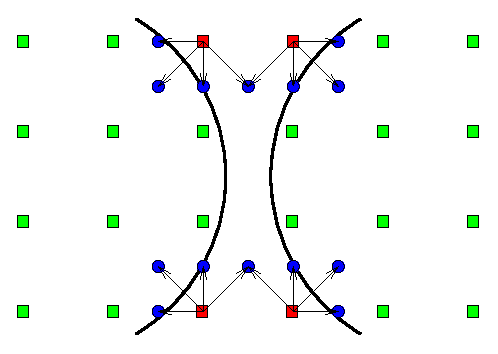
\includegraphics{xfig/colloidclose.eps}
\end{center}
\caption{Two colloids close to contact are missing links in the
region of closest approach owing to a lack of fluid nodes in the
interstice.}
\label{fig:f5}
\end{figure}
Again following Nguyen and Ladd \cite{nl02}, mass conservation is
enforced explicitly using the following procedure. There is a mass
transfer associated with the bounce-back at each link of
$(2w_{c_b}\rho_0 \mathbf{u}_b . \mathbf{c}_b / c_s^2) \Delta x^3$.
The net mass transport into the particle is the sum of this
quantity over all the links, and can be written
\begin{equation}
\Delta M_s = - \frac{2\Delta x^3 \rho_0}{c_s^2}
\Big[ \mathbf{U}.\sum_b w_{c_b} \mathbf{c}_b +
  \mathbf{\Omega} . \sum_b w_{c_b} \mathbf{r}_b \times \mathbf{c}_b \Big].
\end{equation}
For any partilce with a full set of boundary links, both
$\sum_b w_{c_b} \mathbf{c}_b$
and $\sum_b w_{c_b} \mathbf{r}_b \times \mathbf{c}_b$ are zero.
However, if the set of boundary links is imcomplete
(as in Figure~\ref{fig:f5}) $\Delta M_s$ is not zero and
a correction is required. This is again made by redistributing the
excess or deficit of mass over the other existing boundary nodes.
The additional contribution to the bounce-back here is
$-w_{c_b} \rho_0 \Delta M_s/A$, where
$A = \rho_0 \Delta x^3 \sum_b w_{c_b}$ (cf.\ Equation~\ref{eq:q1}).

This contribution
now adds to the velocity-dependent part of the force and torque and
leads to a slightly different form of the drag matrices
\begin{eqnarray}
\boldsymbol{\zeta}^{FU} &=& \frac{-2\rho_0 \Delta x^3}{c_s^2 \Delta t}
\sum_b w_{c_b} (\mathbf{c}_b - \overline{\mathbf{c}_b}) \mathbf{c}_b
\\
\boldsymbol{\zeta}^{F\Omega} &=& \frac{-2\rho_0 \Delta x^3}{c_s^2 \Delta t}
\sum_b w_{c_b} \mathbf{c}_b (\mathbf{r}_b \times \mathbf{c}_b -
\overline{\mathbf{r}_b\times\mathbf{c}_b}),
\\
\boldsymbol{\zeta}^{TU} &=& \frac{-2\rho_0 \Delta x^3}{c_s^2 \Delta t}
\sum_b w_{c_b} (\mathbf{r}_b\times\mathbf{c}_b)
(\mathbf{c}_b - \overline{\mathbf{c}_b}),
\\
\boldsymbol{\zeta}^{T\Omega} &=& \frac{-2\rho_0 \Delta x^3}{c_s^2 \Delta t}
\sum_b w_{c_b} (\mathbf{r}_b\times\mathbf{c}_b)
(\mathbf{r}_b\times\mathbf{c}_b - \overline{\mathbf{r}_b\times\mathbf{c}_b}).
\end{eqnarray}
The mean quantities
\begin{equation}
\overline{\mathbf{c}_b} = \frac{\sum_b w_{c_b} \mathbf{c}_b}{ \sum_b w_{c_b}}
\end{equation}
and
\begin{equation}
\overline{\mathbf{r}_b\times\mathbf{c}_b} =
\frac{\sum_b w_{c_b} \mathbf{r}_b\times\mathbf{c}_b}{\sum_b w_{c_b}}.
\end{equation}
A little algebra will show that both occurances of $\mathbf{c}_b$ and/or
$\mathbf{r}_b\times\mathbf{c}_b$ in the definition of the drag matrices
can be replaced by their deviation from the mean. This provides a
convenient way to compute the drag matrices (maintaining symmetry)
and computing the correct force and torque on the particle when close
to contact.



\subsubsection{Rotational motions}


For a number of applications it is useful to update not only
the psoition of a spherical particle, but its orientation. This
is important, e.g., when considering magnetic particles. The
best way to implementment the required rotations is by
considering quaternions.

A quaternion can be thought of as an extended complex number
\begin{equation}
q = w + xi + yj + zk
\end{equation}
where $i^2 = j^2 = k^2 = -1$ and $ijk = -1$. The norm, or length
of a quaternion is
\begin{equation}
N(q) = (w^2 + x^2 + y^2 + z^2)^{1/2}.
\end{equation}
Addition and subtraction of quaternions proceeds as normal, but
care is required for multiplication, which is associative but not
commutative. If the quaternion is writen as $q = (w, {\bf v})$ where
$\bf{v}$ is a normal 3-vector, then multiplication can be written
\begin{equation}
q_1 q_2 = (w_1 w_2 - {\bf v}_1 . {\bf v}_2, w_1 {\bf v}_2 + w_2 {\bf v}_1
+ {\bf v}_1 \times {\bf v}_2),
\end{equation}
where the usual scalar and vector products are used. Note that the
conjugate of a quaterion $q^\star = (w, -{\bf v})$ so that
$qq^\star = N^2(q)$.
It can be shown that a rotation of an arbitrary vector though an
angle $\theta$ around the unit axis of rotaion $\hat{\bf w}$ can
be represented by the quarternion
\begin{equation}
q = (\cos(\theta/2), \hat{\bf w} \sin(\theta/2))
\end{equation}
which ensures that $N(q) = 1$. If the arbitrary vector is (0, {\bf v}),
then the rotated vector ${\bf v}^{'}$ can be written as
\begin{equation}
(0, {\bf v}^{'}) = q (0, {\bf v}) q^\star
\end{equation}
which can be expanded as
\begin{equation}
{\bf v}^{'} = (1 - \cos\theta)({\bf v}.{\hat{\bf w}) \hat{\bf w} +
{\bf v}\cos\theta} + (\hat{\bf w} \times {\bf v})\sin\theta.  
\end{equation}


\subsection{Colloid-Colloid interactions}

\subsubsection{Lubrication corrections}

\subsubsection{Hard sphere interaction}

Particles do not overlap, i.e., there is always
a hard-sphere interaction which is a function of the separation $h$:
\begin{equation}
v^{hs}(h) = \left\{
\begin{array}{ll}
\infty & h \leq 0,\\
0   & h > 0.
\end{array} \right.
\end{equation}
The hard-sphere interaction does not give rise to a force.


\subsubsection{Soft-sphere interaction}

A simple soft-sphere interaction is available, the basic form
of which is:
\begin{equation}
v^{ss}(r) = \epsilon (\sigma / r)^{\nu},
\end{equation}
where $\epsilon$ sets the energy scale, and $\sigma$ sets the
characteristic width. The steepness of the potential is set by
the exponent $\nu (> 0)$.

To prevent the need for calculation of long-range interactions,
the soft-sphere potential is truncated in a ``cut-and-shift''
approach. This is done in such a way as to smoothly match
both the potential and the force at the cut-off distance
$r_c$. For $r < r_c$ the potential is then
\begin{equation}
v^{ss}(r) - v^{ss}(r_c) - (r - r_c) \left.\frac{d v^{ss}}{dr}\right|_{r=r_c}.
\label{eq_ss_shift}
\end{equation}
Clearly, this potential is not exactly what we first thought of as
soft-sphere. Matching the potential smoothly ensures conservation
of energy, while matching the force smoothly prevents potential
instabilities in the molecular dynamics update.

The soft-sphere potential can be useful as a mechanism to
keep the particles from touching (which risks hard-sphere interactions),
in which case is is possible to compute the interaction as a function
of the separation $h$, instead of $r$. The force between
two particles is computed via the derivative of equation~\ref{eq_ss_shift}
with respect to $r$:
\begin{equation}
\mathbf{F}_{ij}(r) = -\left\{\frac{d v^{ss}(r)}{dr} -
\left. \frac{d v^{ss}(r)}{dr}\right|_{r=r_c} \right\} \mathbf{\hat{r}}_{ij}
\end{equation}
where $\mathbf{\hat{r}}_{ij}$ is the unit vector joining the centre of
particle $i$ to the centre of $j$.



\subsubsection{Leonard-Jones interaction}



\section{Lattice Boltzmann for a Binary Fluid}

\subsection{The Cahn-Hilliard Equation}

\subsection{The Choice of Free Energy}

\subsection{A Second Distribution Function}

\subsection{The Collision}

\subsection{Bounce-Back on Links}




\section{Surfactants}

This section describes the approach taken to study surfactants. Here,
we always adopt the hydrid method, i.e., LB for the hydrodynmic
equations and finite difference for the associated Cahn-Hilliard
equations. Coupling between the two sectors is via the velocity
field and the external force on the fluid computed via the
divergence of the `chemical stress'.

In this model the surfactant appears as a concentration field
$\psi(\mathbf{r};t)$, alongside the compositional order parameter
$\phi(\mathbf{r};t)$ as appears in the binary fluid. There are
two corresponding Cahn-Hilliard equations: first,

\begin{equation}
\partial_t \phi + \partial_\alpha \phi u_\alpha = 
\partial_\alpha M_\phi \partial_\alpha \mu_\phi,
\end{equation}
and second
\begin{equation}
\partial_t \psi + \partial_\alpha \psi u_\alpha = 
\partial_\alpha M_\psi \partial_\alpha \mu_\psi.
\end{equation}

\subsection{Free Energy}

A number of different free energies have been used to study
surfactants [cite Yeomans]. Here, the free energy is based on
that used by van der Graff and van der Sman and others [cite].
There are a number of different contributions to the free
energy density:
\begin{equation}
f = f_\phi + f_\psi +f_1 + f_{ex}.
\end{equation}
The first is exactly that used for the binary fluid, i.e.,
\begin{equation}
f_\phi (\phi, \partial_\alpha\phi) =
{\textstyle \frac{1}{2}} A \phi^2 + {\textstyle \frac{1}{4}} B \phi^4
+ {\textstyle \frac{1}{2}} \kappa (\partial_\alpha \phi)^2.
\end{equation}
The surface tension and the interfacial width are determined from the
choice of parameters $A,B,\kappa$ as before.
The second term in the free energy density
represents the entropic
energy of mixing of the surfactant with the bulk phases
\begin{equation}
f_\psi (\psi) = kT \left[ \psi \ln\psi + (1 - \psi)\ln(1-\psi) \right]
\end{equation}
where the parameter $kT$ sets the energy scale for the whole system.
The surfactant order parameter, $\psi$, is unity for a saturated
interface and zero for a plain interface.

The surfactant lowers the energy of the interface where it is adsorbed
there, represented by the term
\begin{equation}
f_1(\psi, \partial_\alpha \phi) 
= -{\textstyle \frac{1}{2}} \epsilon \psi (\partial_\alpha \phi)^2
  -{\textstyle \frac{1}{2}} \beta  \psi^2 (\partial_\alpha \phi)^2
\end{equation}
where $\epsilon$ and $\beta$ are parameters. Note that only the
first term appears in \cite{vandergraaf}, while the second term is
based on that appearing in, e.g., \cite{diamant}. If $\beta = 0$,
the surfactant profile at the interface is symmetric (so-called
Langmuir adsoption) whereas the term in $\beta$ induces an
asymmetry (Frumpkin adsorption).
Finally,  $f_{ex}$ is [van der Sman claims]
an enthalpic contribution introduced 
to stabilise the interface \cite{theissengompper}
\begin{equation}
f_{ex} (\psi, \partial_\alpha \phi) = {\textstyle\frac{1}{2}} W \psi \phi^2,
\end{equation}
with $W$ a parameter.

\subsection{Chemical potentials}

The respective chemical potentials are obtained from the functional
derivatives of the free energy $\mu_\phi = \delta F / \delta \phi$ and
$\mu_\psi = \delta F / \delta \psi$. We obtain:
\begin{equation}
\mu_\phi =
A\phi + B\phi^3 -\kappa \partial_\alpha^2 \phi
+ W\psi\phi + \epsilon\psi\partial_\alpha^2 \phi
+ \epsilon \partial_\alpha \phi \partial_\alpha \psi
+ 2\beta \psi\partial_\alpha\phi \partial_\alpha \psi
+ \beta \psi^2 \partial_\alpha^2 \phi,
\end{equation}
and
\begin{equation}
\mu_\psi = kT \left[ \ln\psi - \ln(1-\psi) \right]
+ {\textstyle \frac{1}{2}}W\phi^2
- {\textstyle \frac{1}{2}}\epsilon (\partial_\alpha \phi)^2
- \beta\psi (\partial_\alpha \phi)^2.
\end{equation}
As before, the pressure tensor is $P_{\alpha\beta} = p_0\delta_{\alpha\beta}
+ \tilde{P}_{\alpha\beta}$ with the isotropic part being determined as (e.g.,
\cite{theissengompper})
\begin{equation}
p_0 = \phi \mu_\phi + \psi \mu_\psi - f(\phi, \psi, \partial_\alpha \phi).
\end{equation}
There is no closed form for the tensor part, which must be chosen to
comply with the constraint that in mechanical equilibrium
\begin{equation}
\partial_\alpha P_{\alpha\beta} = (\phi\partial_\alpha\mu_\phi +
\psi\partial_\alpha\mu_\psi)\delta_{\alpha\beta}.
\end{equation}
In this way we obtain for the isotropic contribution
\begin{eqnarray}
p_0 = {\textstyle \frac{1}{2}}A\phi^2 + {\textstyle \frac{3}{4}}B\phi^4 
- {\textstyle\frac{1}{2}}\kappa (\partial_\alpha\phi)^2 
- \kappa \phi \partial_\alpha^2 \phi
- kT \ln(1-\psi) + W\psi\phi^2
\nonumber\\
+ \epsilon \phi \partial_\alpha \phi \partial_\alpha \psi
+ \epsilon\phi\psi \partial_\alpha^2 \phi
+ 2 \beta\phi\psi \partial_\alpha \phi \partial_\alpha\psi
+ \beta \phi \psi^2 \partial_\alpha^2 \phi
- {\textstyle\frac{1}{2}} \beta \psi^2 (\partial_\alpha \phi)^2
\end{eqnarray}
and for the tensor part we can have
\begin{equation}
\tilde{P}_{\alpha\beta} =
(\kappa - \epsilon \psi - \beta\psi^2) 
\partial_\alpha \phi \partial_\beta \phi.
\end{equation}

\section{Polar Active Gel}


Here we consider a polar vector field model to study active gels. 
The order parameter is this time a vector $P_\alpha$
(with variable magnitude) as there is no longer head-tail symmetry
in the system as was the case for the ${\bf Q}$ tensor formulation. 
The equation of motion as:
\begin{equation}
\partial_t P_\alpha  \partial_\beta (u_{\beta} + wP_{\beta}) P_{\alpha}
= \lambda D_{\alpha\beta} P_{\beta} - \omega_{\alpha\beta} P_{\beta}
+\Gamma' h_{\alpha}.
\end{equation}

In this equation, $w$ is an active term, due to swimming, which causes
self-advection of the order parameter, while $\lambda$ is a material
dependent constant -- positive for rod-like molecules. If $|\lambda|>1$
the liquid crystalline passive phase is flow-aligning, otherwise it is
flow-tumbling. 

Note that the convection for the Leslie-Ericksen is that the
velocity gradient tensor should be writen $W_{\alpha\beta}
= \partial_\alpha u_\beta$ (and not the other way round, which
is usual).

The molecular field is given by
$h_{\alpha}=-\delta {\cal F}_{\rm pol}/\delta p_{\alpha}$
where ${\cal F}_{\rm pol}$ is the free energy for a polar active nematic,
whose density we can take to be:
\begin{equation}
f =  \frac{\alpha_2}{2} |{\mathbf P}|^2 + \frac{\alpha_4}{4}|{\mathbf P}|^4
+ \frac{K}{2}\left(\partial_\alpha P_{\beta}\right)^2 + 
\frac{K_{LC}}{2}\left[\partial_\alpha (P_{\beta}P_{\gamma})\right]^2 
\end{equation}
where $K$ and $K_{LC}$ are elastic constants, $\alpha_4>0$, and $\alpha_2$ 
can be positive (isotropic phase) or negative (polar nematic phase).

The molecular field is explicitly given by:
\begin{equation}
h_{\alpha}=-\alpha_2 P_{\alpha} -\alpha_4 P_{\alpha} P_{\beta}P_{\beta}+
K \partial_{\beta}\partial_{\beta} P_{\alpha}+2 K_{LC}
P_{\gamma}\partial_{\beta}\partial_{\beta} (P_{\gamma}P_{\alpha}).
\end{equation}


The Navier-Stokes equation is:
\begin{equation}
\rho \left(\partial_t+v_{\beta}\partial_{\beta}\right) v_{\alpha} =
\partial_{\beta} \Pi_{\alpha\beta} 
+\eta \partial_{\beta}\partial_{\beta} v_{\alpha}.
\end{equation}


The stress tensor this time is 
\begin{eqnarray}
\Pi_{\alpha\beta} =
\frac{1}{2}\left(P_\alpha h_\beta - P_\beta h_\alpha \right)
- \lambda\left( (P_\alpha h_\beta + P_\beta h_\alpha)/2 
- (1/3)P_\gamma P_\gamma \delta_{\alpha\beta} \right)
\\
-  \zeta ( P_\alpha P_\beta - (1/3)P_\gamma P_\gamma \delta_{\alpha\beta})
- K \partial_\alpha P_\gamma \partial_\beta P_\gamma.
\end{eqnarray}
The active term in the stress tensor, proportional
to $\zeta$, has the same form for apolar and polar active gels. 

\section{Code Design}

\subsection{Some Comments}

In designing a code in C the main object of which is to do high
performance computing, there are some inevitable tensions with
software engineering best-practice. In particular, complete
encapsulation of data in the spirit of using abstract data types
tends to cause problems of performance.

For example, encapsulation of the lattice Boltzmann distribution
$f_i$, together with appropriate ``get'' and ``set'' functions for
access when approapriate, is possible. There could then be a
complete separation of interface and implementation of the
distribution (other than that each individual $f_i$ is represented
by a \texttt{double}). However, experience suggests that
this imposes severe impediment to optimisation and hence
unacceptable performance degradation.

Schemes do exist by which one can approximate the object
oriented programming style in C, and so achieve a separation
of interface and implementation. However, this tends to put
a heavy burden on the use of \texttt{void} pointers, itself
a recipe for possible disaster. A truly object-oriented
language such as Java would be preferable.

So, for the time being, some relaxation of encapsulation is required.
Exposing a pointer to the distributions which allows them to be accessed
directly where required. This can be done merely by declaring the
necessary variables \texttt{extern}. In practice, such deviations
from encapsulation can be minimised in the lattice sector of the
code. In particlar, \texttt{extern} declarations should not be
required in \texttt{main()}, i.e., it should be able to write a
new application without worrying about details of implementation.

\subsubsection{Objects}

Somewhat more difficult is the part of the code involving
colloids, which would really favour a truly object-oriented
approach.

\subsubsection{Serial and parallel}

The design decission has been taken to support execution of the
code in both serial and parallel. The default compilation
assumes that a serial executable is required, while  MPI code
is introduced via C-preprocessor directives (\texttt{-D\_MPI\_}).


There is no shared memory inplementation at this time.


\subsection{Structural Components: \texttt{MPI\_COMM\_WORLD}}


\subsection{Coordinate System: \texttt{MPI\_CARTESIAN\_COMMUNICATOR}}


\begin{figure}
\begin{center}
%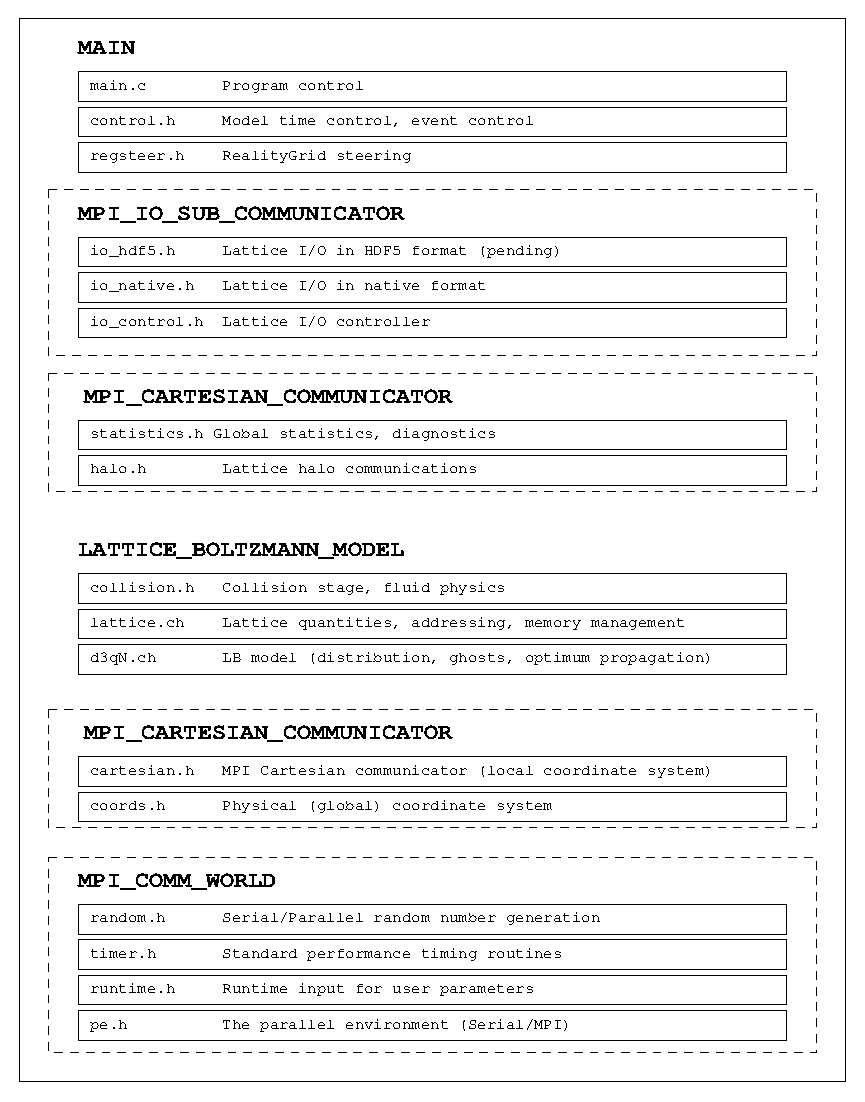
\includegraphics{xfig/sketch.eps}
\end{center}
\caption{A scheme by which different parts of the code might be
encapsulated and in such a way to allow reliable development and
testing. As this is C, will do not adopt a truly ``object'' langauge.
Broadly, different modular parts should only depend on stuff above
in the diagram. So, at the top, there is the parallel environment
where communication occurs within MPI\_COMM\_WORLD. Built on top
of this is the Cartesian Communicator responsible for halo swaps
and so forth. The LE code may have a separate Communicator again. 
(There's an argument to say the diagram should be the other way up!)}
\end{figure}



\section{Code Implementation}

\subsection{Stuff}

\subsection{Coordinate System}

\subsubsection{The global coordinate system}

The user specifies the system size in lattice units at run time,
which sets the extent of memory which must be allocated for the
Cartesian lattice. The extent of the physical coordinate system
then reflects the lattice size directly (see Figure \ref{fig_c1}). 
Each lattice site, or node,  has coordinates corresponding to its
integer position in the system and can be thought of as being
at the centre of a control volume one lattice unit on a side.
This means that the nominal edges of the
system are offset from the lattice sites themselves by half a
lattice unit in each direction.


\begin{figure}[h]
\begin{center}
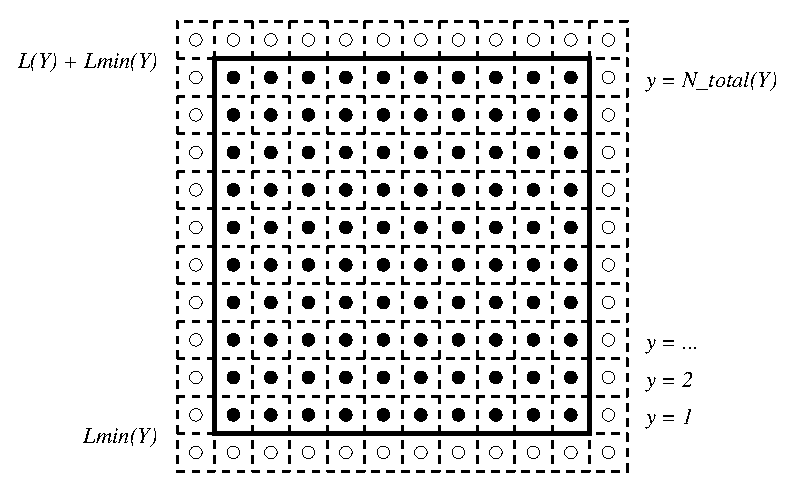
\includegraphics{xfig/fig_c1.eps}
\end{center}
\caption{The global Cartesian coordinate system reflects the choice
of lattice size; lattices sites are located at
$x=1, \ldots, x = N_{total}$ and so on in each coordinate direction
(the Figure only shows the labels in the $y-$direction for simplicity).
In the Figure, the lattice sites in the domain proper are the full
circles; halo sites, which are used to effect periodic boundary
conditions, are included as open cirles}
\label{fig_c1}
\end{figure}

For particles, the centres of which can move continuously across the
lattice, the extents of the global coordinate system are then
$L_{min} < x < L + L_{min}$ and so on.

\subsubsection{Addressing the lattice: the local coordinate system}


\subsection{Solid walls}

General solid objects which are fixed for the duration of
the simulation, such as porous media, can be defined
by assigning solid/fluid status to each lattice node. 
The links required between solid and fluid nodes can
then be identified for the given model.

\textit{Comment.} In general, a solid object will not
affect the periodic nature of the simulation. A general
solid object cannot move, i.e., the boundary velocity
must be zero.

\textit{Special case.} In the case where the solid object
represents a flat boundary wall at the edge of the system
in one or more directions, the periodicity is broken in
the corresponding directions.



%%%%%%%%%%%%%%%%%%%%%%%%%%%%%%%%%%%%%%%%%%%%%%%%%%%%%%%%%%%%%%%%%%%%%%%%%%%%%
% LE Implementation
%%%%%%%%%%%%%%%%%%%%%%%%%%%%%%%%%%%%%%%%%%%%%%%%%%%%%%%%%%%%%%%%%%%%%%%%%%%%%

\subsection{Lees Edwards Sliding Period Boundary Conditions}

\subsubsection{The LE module}

\subsubsection{Distributions crossing the LE planes}

With the planes conceptually half-way between lattice sites, the
propagation moves some of the distributions (namely, those with
$c_x = \pm1$) between different sliding blocks. While the collision
stage is unaffected, action must be taken to adjust these
distributions when the LE boundary conditions are active. This
is done in a two-stage process described by Adhikari \textit{et al.}
\cite{adhikari_desplat}, implemented between the collision and
propagation.

\textbf{a. Reprojection} The post-collision distributions with
$c_x = \pm 1$ at sites adjacent to a boundary are modified to
take account of the velocity jump $\pm u^{LE}_y$ between the sliding
blocks. In terms of the hydrodynamic moments we have:
\begin{eqnarray}
\rho &\rightarrow& \rho', \\
\rho u_\alpha &\rightarrow& (\rho u_\alpha)' \pm \rho' u^{LE}_\alpha, \\
S_{\alpha\beta} &\rightarrow&
S'_{\alpha\beta} \pm (\rho u_\alpha)' u^{LE}_\beta
\pm (\rho u_\beta)' u^{LE}_\alpha + \rho' u^{LE}_\alpha u^{LE}_\beta.
\end{eqnarray}
If we work with the changes to the moemnts, then the density is
unaffected $\delta\rho =  0$, the velocity is changed by
$\delta u_\alpha = \pm u^{LE}_\alpha$, with an analogous expression for
the change in the stress
\begin{equation}
\delta S_{\alpha\beta} =
\pm (\rho u_\alpha)' u^{LE}_\beta
\pm (\rho u_\beta)' u^{LE}_\alpha + \rho' u^{LE}_\alpha u^{LE}_\beta.
\end{equation}
We can then work out the change in the distributions by reprojecting
via Eq.\ref{eq:}, i.e.,
\begin{equation}
f_i \rightarrow f_i' + w_i \Bigg(
\frac{\rho \delta u_\alpha c_{i\alpha}}{c_s^2} +
\frac{\delta S_{\alpha\beta}Q_{i\alpha\beta}}{2c_s^4} \Bigg).
\end{equation}
A similar set of expressions are given for the order parameter
distributions in Adhikari \textit{et al.} \cite{adhikari_desplat}.

\textbf{b. Interpolation of reprojected distributions}
As the sliding blocks are displaced continuously with
$\delta y = u_y^{LE}t$, which is not in general a whole number of
lattice spacings, an interpolation is also required before
propagation can take place. Consider the situation (Fig.~\ref{fig_le2}) from
a stationary frame where the frame above has translated a small
distance to the right ($\delta y < \Delta y$). In the stationary frame
we must interpolate the ditributions with $c_x = 1$ to a
`departure point' from which the propagation will move the
distribution exactly to the appropriate lattice site in the moving
frame. Schemeatically,
\begin{equation}
f_i'(x, y + \delta y, z) = 
 (1 - \delta y) f_i^\star(x, y, z) +
\delta y f_i^\star(x, y + \Delta y, z),
\end{equation}
where $f_i'$ here represents the interpolated value and $f_i^\star$
is the reprojected post-collision quantity.

In the case where the displacement $\delta y > 1$, the relevant
lattice sites involved in the interpolation are displaced to the right
by the integral part of $\delta y$, while the relative weight given to
the two sites involves
the fractional part of $\delta y$. To take account of the periodic
boundary conditions
in the $y$-direction, all displacements are modulo $L_y$.


\begin{figure}[h]
\begin{center}
%\includegraphics{xfig/fig_le2.eps}
\end{center}
\caption{Schematic diagram showing interpolation of distributions in the
stationary plane (below) in preparation for propagation into the moving
frame (above). For a small displacement $\delta y = u^{LE} t$, the
interpolation takes place between lattice sites in the stationary frame
(green, left). Propogation from the interpolated positions (red) can
then take place into the moving frame (right).}
\label{fig_le2}
\end{figure}


In parallel, exactly the same calculation is undertaken. However,
communication is required to take account of the processor
decomposition in the $y$-direction. This requires the identification
of the two processes which hold the relevant information as a function
of displacement. 

Note that the interpolated values are stored in the appropriate lattice
site in the rest frame that ensures the normal propagation stage moves all
distributions to the correct destination in memory.

\subsubsection{Order parameter gradients}

When the order parameter gradient is computed at a given point
near the LE boundaries, the stencil may extend out of the stationary
frame. The process of interpolation is slightly different to that
for the distributions.

Here, we need to interpolate values in the moving frame to the position
which is seen by the rest frame. Figure~\ref{fig_le3} shows a five-point
stencil to calculate the gradient at the central point $(x,y,z)$ in the
rest frame. An interpolation of the $\phi$-field of the form
\begin{equation}
\phi'(x + \Delta x, y - \delta y, z) =
\delta y \phi(x + \Delta x,  y - \Delta y, z) + 
(1 - \delta y) \phi(x + \Delta x, y, z)
\end{equation}
must then take place. In practice, the interpolated values are stored
in the offset buffer. As the gradient calculation requires $\phi$
values in the halo regions, interpolated values for the buffer halo
region are also required.

\begin{figure}[h]
\begin{center}
%\includegraphics{xfig/fig_le3.eps}
\end{center}
\caption{Schematic diagram showing a five-point stencil to compute a
gradient at the central point in the stationary frame. The upper point
of the stencil is in the moving frame and so must be interpolated to
the correct position (red sites).}
\label{fig_le3}
\end{figure}

In parallel, the interpolation requires data from at most two adjacent
processes in the along-plane $y-$direction as long as the $\phi$ halo
regions are up-to-date. The rank of the processes involved is
determined by the displacement $\delta y$ as a function of time.


\subsubsection{Velocities and finite-difference fluxes}

For the finite-difference implementation, the velocity field at
the cell boundaries is required. At the planes, this means an
interpolation which takes the same form as that for
$\phi$ is needed.

In computing the advective fluxes between cells, we must then
allow for the presence of the planes. This is done by computing
separately the 'east' and 'west' face fluxes in the $x$-direction
(the flux that crosses the plane). Away from the planes, face-flux
uniqueness $f_{ijk}^e = f_{i+1jk}^w$ ensures conservation of order
parameter. However, at the planes, the non-linear conbination of
velocity field and order parameter field does not in general give
rise to consistent fluxes. In order to restore conservation, we
reconcile east and west face fluxes at the plane by taking an
average
\begin{eqnarray}
f_{ijk}^{e\star}&=&{\textstyle\frac{1}{2}}(f_{ijk}^e + f_{i+1j'k}^w),\quad 
f_{i+1j'k}^w  = \delta y f_{i+1 j-1 k}^w + (1 - \delta y) f_{i+1jk}^w,\\
f_{i+1 j k}^{w\star} &=& {\textstyle\frac{1}{2}}(f_{ij'k}^e + f_{i+1jk}^w),\quad
f_{ij'k}^e = (1 - \delta y) f_{ijk}^e + \delta y f_{ij+1k}^e.
\end{eqnarray}
In this way, we average the east face flux in the rest frame $f_{ijk}^e$
with the interpolated value of the west face flux in the moving frame
$f_{i+1j'k}^w$, and vice-versa. One can then easily show that when
integrated over the length of the plane, the average fluxes are
consistent, i.e.,
\begin{equation}
\sum_j (f_{ijk}^{e\star} - f_{i+1jk}^{w\star}) = 0 \quad\forall k,
\end{equation}
thus ensuring order parameter conservation.

A similar correction is required when computing the force on the fluid
directly via the divergence of the thermodynamic stress
$F_\alpha = \nabla_\beta P_{\alpha\beta}^{th}$. This is implementated
by computing fluxes of momentum at cell faces in each direction, and
then taking the divergence to compute the force. At the planes, an
averaging procedure is again used to ensure conservation of momentum.

%%%%%%%%%%%%%%%%%%%%%%%%%%%%%%%%%%%%%%%%%%%%%%%%%%%%%%%%%%%%%%%%%%%%%%%%%%%%%
% End LE implementation
%%%%%%%%%%%%%%%%%%%%%%%%%%%%%%%%%%%%%%%%%%%%%%%%%%%%%%%%%%%%%%%%%%%%%%%%%%%%%


\vfill
\pagebreak

\section{Code Interface}

\subsection{The Parallel Environment}

\texttt{\#include ``pe.h''}

As the code is to be available in both serial and parallel versions,
it is desirable to abstract the basic environment to some extent.
The parallel environment is intended to support MPI communication
within \texttt{MPI\_COMM\_WORLD}, or fall back to a minimally
consistent picture in serial (i.e., rank zero is the single process).

\texttt{void pe\_init(int argc, char ** argv)}\\
Responsible for initialisation of MPI, and hence must be first
execuatable statement. The arguments are those to \texttt{main}
which will be passed through to \texttt{MPI\_Init()}.

\texttt{int pe\_rank(void)}\\
Returns the process rank in \texttt{MPI\_COMM\_WORLD}, or 0 in
serial.

\texttt{int pe\_size(void)}\\
Returns the number of processes in \texttt{MPI\_COMM\_WORLD}, or
1 in serial.

\texttt{void pe\_finalise(void)}\\
Responsible for \texttt{MPI\_Finalize()}, and must be the last
executable statement.

\texttt{void info(const char * fmt, ...)}\\
Behaves like \texttt{printf}, but only produces output on the
root process.

\texttt{void verbose(const char * fmt, ...)}\\
Behaves as \texttt{printf} and reports the rank of the
calling process in \texttt{MPI\_COMM\_WORLD}.

\texttt{void fatal(const char * fmt, ...)}\\
Prints an error message and identifies
the rank of the calling process before terminating the program.


\subsection{Run Time Input}

\texttt{\#include ``runtime.h''}

The ability to set a wide range of parameters at run time is
very convenient, and is supported via an input file in which the
user specifies parameters as key value pairs. The code maintains
a list of key value pairs from which the user can retrieve the
appropriate values for given keys.


\texttt{void RUN\_read\_input\_file(const char * input\_file\_name)}\\
This reads the named input file and sets up the list of keys.

\texttt{int RUN\_get\_double\_parameter(const char *key, double * value)}\\
Set the \texttt{value} associated with \texttt{key}, if present. The number
of key matches found is returned (i.e., 0 or 1).

\texttt{int RUN\_get\_int\_parameter(const char * key, int * value)}\\
Set the \texttt{value} associated with \texttt{key}, if present. The
number of key matches is returned.

\texttt{int  RUN\_get\_string\_parameter(const char * key, char * value)}\\
Set \texttt{value} to the string assocaited with \texttt{key}, if
present. Returns the number of key matches found.

\texttt{int  RUN\_get\_int\_parameter\_vector(const char * key, int v[])}\\
If \texttt{key} is present, set the associated 3-vector of integers.
Returns the number of key matches found. 

\texttt{int  RUN\_get\_double\_parameter\_vector(const char * key,
double v[])}\\
If \texttt{key} is present, set the associated 3-vector of doubles.
Returns the number of key matches found.

\textit{Comment:} We probably need a function to report unused keys, so
the user can be alerted if a key has unexpectedly been ignored.


\subsection{Random Number Generators}

\texttt{\#include ``ran.h''}

Note that the random number generation in parallel is
decomposition dependent.

\texttt{void rand\_init(void)}\\
Responsible for initialising RNG state.

\texttt{double rand\_serial\_uniform(void)}\\
Return a single variate uniformly distributed on $[0,1]$ from
the serial generator.

\texttt{double rand\_serial\_gaussian(void)}\\
Return a single variate with Gaussian distribution about zero
and having unit variance from the serial generator.

\textit{double rand\_parallel\_uniform(void)}\\
Return a single variate uniformly distributed on $[0,1]$
from the serial generator.

\texttt{double rand\_parallel\_gaussian(void)}\\
Return a single variate with Gaussian distribution about zero
and having unit variance from the parallel generator.

\textit{Comment:} The serial generator will produce the
same sequence on any MPI process, while the parallel generator
will produce different sequences. The latter is intended for
generating, specifically, fluctuations, where the need for
decomposition-independance is questionable.



\subsection{Timers}

\texttt{\#include ``timer.h''}

Performance figures require timing for different sections
of the code. The code provides a set of routines to time
standard and user-defined sections of code. Timers are
started and stopped by call to the appropriate routines.

\texttt{TIMER\_init()}\\
This initialises all the timers to zero (e.g., at the start of
the program).

\texttt{TIMER\_start(const int t\_id)}\\
Start the given timer.

\texttt{TIMER\_stop(const int t\_id)}\\
Stop the given timer.

\texttt{TIMER\_statistics(void)}\\
Prints the current state of all the active timers to standard
output on the root process in a digestible form. In serial,
the minimum, maximum, and mean time for each timer is reported
in seconds (based on the number of start/stop cycles). In
parallel, the same figures are computed on each process and the
result of the corresponding \texttt{MPI\_Reduce()} operation is
printed on the root process.

The code provides a number of timers which would time standard
parts of the code, e.g., \texttt{t\_id = TIMER\_TOTAL} for the
total execution time, and a number of spare timers for users to
use at will.


\textit{Comment:}
No intra-run variance (i.e., between time steps) is provided, as the
calculation required is considerably more complex to generalise, and
requires memory proportional to the number of time steps used.


\textit{Comment:}
Two macros, \texttt{TIMER\_START()} and \texttt{TIMER\_STOP()} are
provided to insert calls to the above functions for optional timing
of performance-sensitive regions
of the code in conjunction with the preprocessor flag
\texttt{-D\_TIMING\_MACRO\_ON\_}.


\subsection{Model Time Control}

This provides time step control, event frequency (?)

\texttt{void init\_control(void)}\\
Initialise time controls.

\texttt{int get\_step(void)}\\
Return the current model time step.

\texttt{int next\_step(void)}\\
Increments the current time step. Returns number of steps left
to run (i.e., 0 when finished).



\subsection{Coordinate System}

\texttt{\#include ``coords.h''}

A three-dimensional Cartesian coordinate system is used throughout,
with the exact system size usually chosen by the user at run time.
The symbolic constants \texttt{X}, \texttt{Y}, and \texttt{Z} are
used to identify the coordinate directions.

This also provides access to the MPI Cartesian Communicator which
is responsible for most communication in the model.

\texttt{int N\_total(const int dim)}\\
Returns the total number of lattice sites in the given Cartesian direction.

\texttt{double L(const int dim)}\\
Returns the length of the system in the given Cartesian direction
(which is the same as the number of lattice sites).

\texttt{double Lmin(const int dim)}\\
Returns coordinate position of left-hand edge of system in given
Cartesian direction.

\texttt{int is\_periodic(const int dim)}\\
Returns 1 if given Cartesian direction is periodic, else 0.

\texttt{void cart\_init(void)}\\
Responsible for setting up the Cartesian decomposition.

\texttt{int cart\_rank(void)}\\
Returns rank in the Cartesian communicator.

\texttt{MPI\_Comm cart\_comm(void)}\\
Returns the MPI Communicator handle for the Cartesian communicator.

\texttt{int cart\_size(const int dim)}\\
Returns the size of the Cartesian communicator grid in the given
coordinate direcxtion.

\texttt{int cart\_coord(const int dim)}\\
Returns the coordinate of the current process in the Cartesian
Communicator.

\texttt{int cart\_neigh(const int dir, const int dim)}\\
Returns the rank of the neighbouring process in the
Cartesian communicator.


\subsection{Colloids}

\texttt{\#include ``colloids.h''}

These functions provide the basic interface for use
of colloidal particles in the code.

\subsubsection{Colloid structure}

The basic colloid struct is defined ...
 

\subsubsection{Colloid interface}

\texttt{void colloids\_init(void)}\\
Call once for initialisation. This initialises the cell list,
so the coordinate system must be initialised via a call to
\texttt{coords\_init()} first.

\texttt{void colloids\_finish(void)}\\
Call once for finalisation. Frees all colloid-related memory.

\texttt{Colloid * allocate\_colloid(void)}\\
Returns a pointer to a newly allocated \texttt{Colloid} object
or fails gracefully.

\texttt{void free\_colloid(Colloid * p\_colloid)}\\
Deallocates all memory associated with \texttt{p\_colloid} or
fails gracefully.

\texttt{struct c\_link allocate\_boundary\_link(void)}\\
Returns a pointer to a newly allocated colloid boundary
link or fails gracefully.

\texttt{void free\_boundary\_link(struct c\_link *)}\\
Deallocates memory associated with a link or fails gracefully.

\texttt{void colloids\_memory\_report(void)}\\
The module keeps track of how much memory has been allocated in
total for colloids and boundary links. This reports the current
usage.

\texttt{get\_Ncell\_total()}\\

\texttt{get\_Ncell\_local()}\\

\texttt{Colloid * cell\_get\_colloid(int i, int j, int k)}\\
This returns a pointer to the Colloid at the head of the list at
cell list location (i, j, k) or \texttt{NULL} if there is none.

\texttt{void cell\_insert(Colloid * p\_colloid)}\\
This inserts a colloid at the head of the appropriate list
depending upon its position. This is the only way a colloid
can be added to the list.

\texttt{update\_cells(void)}\\
Performs the update of the cell list in response to updated
particle positions.

\texttt{IVector cell\_coords(FVector r)}\\




\subsection{Speculation}

\subsection{The Free Energy}

It is imagined that a single file will encapsulate all the details
of a given free energy. The interface for different choices of
free energy should be the same.


\texttt{FE\_init()}

Responsible for querying the runtime input key value pair list to
find appropriate user parameters for the free energy, or
falling back to default values.


\texttt{double FE\_get\_sigma()}

Return the surface tension. There should be a similar routine
for the interfacial thickness.

\texttt{double FE\_get\_mu(const type location)}

Return the chemical potential at the single lattice
node \texttt{location}.

\textit{Comment:} The computation of quantities such as the chemical
potential will a) affect performance and b) require halo values of
the order parameter (depending on the highest derivative
in the order parameter present). Performance here should be the
first consideration, so this needs to be handled with care.


\texttt{double pchem[ND][ND] FE\_get\_pchem(const type location)}

Return the chemical stress ${\cal P}_{\alpha\beta}$ at the
given location.

\textit{Comment:} This is an $nd \times nd$ matrix, where $nd$ is
the number of dimensions. If we are to provide explicit support for
D2Q9, \texttt{ND} will be 2, otherwise 3.





\section{Implementation Notes}

\subsection{Serial Version}

\subsection{Efficiently Scaling Parallel Computing}

We should be thinking about the 100,000 processor regime, and
correspondingly large system sizes. To avoid embarrassment in this regime,
some issues which don't usually arise are relevant, for example:

\begin{enumerate}
\item
Large integer quantities such as
\begin{verbatim}
   N_total.x*N_total.y*N_total.z
\end{verbatim}
are likely to cause integer overflow (if default integers are 4 byte).
\item
Local data structures whose size is proportional
to the number of processors are contraindicated, e.g.,
anything like
\begin{verbatim}
p = (foo *) malloc(nprocs*sizeof(foo));
\end{verbatim}
is to be avoided. At the moment, we are in good shape on this
(apart from some functions in \texttt{misc.c}).
\item
I/O is likely become a very important issue, so may need to think
more about this.
\item
We should probably introduce a standard set of benchmarks which can
be scaled up in some systematic way, so that we can keep track of
performance over time.

\end{enumerate}


\section{Model Details}

\subsection{D2Q9}

These are the eigenvalues and eigenvectors of the collision
matrix used for D2Q9


\begin{table}
\begin{tabular}{|l|r|rrrrrrrrr|r|l|}
\hline\hline
$M^a$ & & \multicolumn{9}{c|}{$m_i^a$} & $N^a$  &\\
\hline
$\rho$ & - & 1 &  1 &  1 &  1 &  1 &  1 &  1 &   1 &  1 & 1 &$\mathbf{1}$ \\
\hline
$\rho c_{ix}$ & - & 0 &  1 &  1 & 1 & 0 &  0 & -1 &  1 & -1 & 3 & $c_{ix}$ \\
\hline
$\rho c_{iy}$ & - & 0 & 1 &  0 &  -1 &  1 &  -1 & 1 & 0 & -1 & 3  &$c_{iy}$ \\
\hline
$Q_{xx}$ & 1/3 & -1 &  2 &  2 & 2 & -1 & -1 & 2 & 2 & 2 & 9/2 
& $c_{ix} c_{ix} - c_s^2$ \\
\hline
$Q_{xy}$ & - & 0 &  1 & 0 & -1 & 0 & 0 & -1 & 0 & 1 & 9 & $c_{ix} c_{iy}$ \\
\hline
$Q_{yy}$ & 1/3 & -1 &  2 & -1 & 2 & 2 & 2 & 2 & -1 & 2 & 9/2
& $c_{iy} c_{iy} - c_s^2$ \\
\hline\hline
$\chi^1$ & - &  1 & 4 & -2 & 4 & -2 & -2 & 4 & -2 & 4 & 1/4 & $\chi^1$ \\
\hline
$J_{ix}$ & - & 0 &  4 & 0 & -4 & -2 & 2 & 4 & 0 & -4 & 3/8
& $\chi^1 \rho c_{ix}$\\
\hline
$J_{iy}$ & - & 0 & 4 & 0 & -4 & -2 & 2 & 4 & 0 & -4 & 3/8
& $\chi^1 \rho c_{iy}$\\
\hline\hline
$w_i$ & 1/36 & 16 & 1 & 4 & 1 & 4 & 4 & 1 & 4 & 1 & & $w_i$\\
\hline\hline
\end{tabular}
\end{table}

\subsection{D3Q15}

These are the eigenvalues and eigenvectors of teh collision
matrix used for D3Q15


\begin{table}
\begin{tabular}{|l|r|r|rrrrrr|rrrrrrrr|r|l|}
\hline\hline
$M^a$ & & \multicolumn{15}{c|}{$m_i^a$} & $N^a$  &\\
\hline
$\rho$ & - &
 1 &  1 &  1 &  1 &  1 &  1 &  1 &  1 &  1 &  1 &  1 &  1 &  1 &  1 &  1 &
1 &$\mathbf{1}$ \\
\hline
$\rho c_{ix}$ & - &
 0 &  1 & -1 &  0 &  0 &  0 &  0 &  1 & -1 &  1 & -1 &  1 & -1 &  1 & -1 &
3  & $c_{ix}$ \\
\hline
$\rho c_{iy}$ & - &
 0 &  0 &  0 &  1 & -1 &  0 &  0 &  1 &  1 & -1 & -1 &  1 &  1 & -1 & -1 &
3  &$c_{iy}$ \\
\hline
$\rho c_{iz}$ & - &
 0 &  0 &  0 &  0 &  0 &  1 & -1 &  1 &  1 &  1 &  1 & -1 & -1 & -1 & -1 &
3  & $c_{iz}$ \\
\hline
$Q_{xx}$ & 1/3 &
-1 &  2 &  2 & -1 & -1 & -1 & -1 &  2 &  2 &  2 &  2 &  2 &  2 &  2 &  2 &
9/2  & $c_{ix} c_{ix} - c_s^2$ \\
\hline
$Q_{yy}$ & 1/3 &
-1 & -1 & -1 &  2 &  2 & -1 & -1 &  2 &  2 &  2 &  2 &  2 &  2 &  2 &  2 &
 9/2 & $c_{iy} c_{iy} - c_s^2$ \\
\hline
$Q_{zz}$ & 1/3 &
-1 & -1 & -1 & -1 & -1 &  2 &  2 &  2 &  2 &  2 &  2 &  2 &  2 &  2 &  2 &
 9/2 & $c_{iz} c_{iz} - c_s^2$ \\
\hline
$Q_{xy}$ & - &
 0 &  0 &  0 &  0 &  0 &  0 &  0 &  1 & -1 & -1 &  1 &  1 & -1 & -1 &  1 &
9  & $c_{ix} c_{iy}$ \\
\hline
$Q_{yz}$ & - &
 0 &  0 &  0 &  0 &  0 &  0 &  0 &  1 &  1 & -1 & -1 & -1 & -1 &  1 &  1 &
9  & $c_{iy} c_{iz}$ \\
\hline
$Q_{zx}$ & - &
 0 &  0 &  0 &  0 &  0 &  0 &  0 &  1 & -1 &  1 & -1 & -1 &  1 & -1 &  1 &
9  & $c_{iz} c_{ix}$ \\
\hline\hline
$\chi^1$ & - &
-2 &  1 &  1 &  1 &  1 &  1 &  1 & -2 & -2 & -2 & -2 & -2 & -2 & -2 & -2 &
1/2 & $\chi^1$ \\
\hline
$J_{ix}$ & - &
 0 &  1 & -1 &  0 &  0 &  0 &  0 & -2 &  2 & -2 &  2 & -2 &  2 & -2 &  2 &
3/2 & $\chi^1 \rho c_{ix}$\\
\hline
$J_{iy}$ & - &
 0 &   0 &  0 &  1 & -1 &  0 &  0 & -2 & -2 &  2 &  2 & -2 & -2 &  2 &  2 &
3/2 & $\chi^1 \rho c_{iy}$\\
\hline
$J_{iz}$ & - &
 0 &   0 &  0 &  0 &  0 &  1 & -1 & -2 & -2 & -2 & -2 &  2 &  2 &  2 &  2 &
3/2 & $\chi^1 \rho c_{iz}$\\
\hline
$\chi^3$ & - &
 0 &   0 &  0 &  0 &  0 &  0 &  0 &  1 & -1 & -1 &  1 & -1 &  1 &  1 & -1 &
9 & $c_{ix} c_{iy} c_{iz}$ \\
\hline\hline
$w_i$ & 1/72 &
$16$ & 8 & 8 & 8 & 8 & 8 & 8 & 1 & 1 & 1 & 1 & 1 & 1 & 1 & 1 &
 & $w_i$\\
\hline\hline
\end{tabular}
\end{table}


\subsection{D3Q19}

\begin{table}
\begin{tabular}{|l||r|rrrrrr|rrrr|rrrr|rrrr|r||}
\hline\hline
$M^a$ & \multicolumn{19}{c||}{$m_i^a$} & $N^a$\\
\hline
$\rho $ & 1 &  1 &  1 &  1 &  1 &  1 &  1 & 
         1 &  1 &  1 &   1 &  1 &  1 &  1 & 1 & 1 & 1 & 1 & 1
& 1\\
\hline
$\rho c_{ix}$ & 0 &  1 &  -1 &  0 &  0 &  0 &  0 & 
         1 &  1 &  -1 &   -1 &  1 &  1 &  -1 & -1 & 0 & 0 & 0 & 0
& 3 \\
\hline
$\rho c_{iy}$ & 0 &  0 &  0 &  1 &  -1 &  0 &  0 & 
         1 &  -1 &  1 &   -1 &  0 &  0 &  0 & 0 & 1 & 1 & -1 & -1
& 3\\
\hline
$\rho c_{iz}$ & 0 &  0 &  0 &  0 &  0 &  1 &  -1 & 
         0 &  0 &  0 &   0 &  1 &  -1 &  1 & -1 & 1 & -1 & 1 & -1
& 3\\
\hline
$Q_{ixx}$ & -1 &  2 &  2 &  -1&  -1 &  -1 &  -1 & 
         2 &  2 &  2 &   2 &  2 &  2 &  2 & 2 & -1 & -1 & -1 & -1
& 9/2\\
\hline
$Q_{iyy}$ & -1 &  -1 &  -1 &  2&  2 &  -1 &  -1 & 
         2 &  2 &  2 &   2 &  -1 &  -1 &  -1 & -1 & 2 & 2 & 2 & 2
& 9/2\\
\hline
$Q_{izz}$ & -1 &  -1 &  -1 &  -1&  -1 &  2 &  2 & 
         -1 &  -1 &  -1 &   -1 &  2 &  2 & 2 & 2 & 2 & 2 & 2 & 2
& 9/2\\
\hline
$Q_{ixy}$ & 0 &  0 &  0 &  0&  0 &  0 &  0 & 
          1 &  -1 &  -1 &    1 &  0 &  0 & 0 & 0 & 0 & 0 & 0 & 0
& 9\\
\hline
$Q_{ixz}$ & 0 &  0 &  0 &  0&  0 &  0 &  0 & 
          0 &   0 &   0 &   0 &  1 & -1 & -1 & 1 & 0 & 0 & 0 & 0
& 9\\
\hline
$Q_{iyz}$ & 0 &  0 &  0 &  0&  0 &  0 &  0 & 
          0 &   0 &   0 &   0 &  0 & 0 & 0 & 0 & 1 & -1 & -1 & 1
& 9\\
\hline\hline
$\chi^1$ & 0 &  1 &  1 &  1 &  1 &  -2 &  -2 & 
         -2 &  -2 &  -2 &  -2 &  1 &  1 & 1 & 1 & 1 & 1 & 1 & 1
& 3/4\\
\hline
$\chi^1 \rho c_{ix}$ & 0 &  1 &  -1 &  0&  0 &  0 &  0 & 
         -2 &  -2 &  2 &  2 &  1 &  1 & -1 & -1 & 0 & 0 & 0 & 0
& 3/2\\
\hline
$\chi^1 \rho c_{iy}$ & 0 &  0 &  0 &  1&  -1 &  0 &  0 & 
         -2 &  2 &  -2 &  2 &  0 &  0 & 0 & 0 & 1 & 1 & -1 & -1
& 3/2\\
\hline
$\chi^1 \rho c_{iz}$ & 0 &  0 &  0 &  0&  0 &  -2 &  2 & 
         0 &  0 &  0 &  0 &  1 &  -1 & 1 & -1 & 1 & -1 & 1 & -1
& 3/2\\
\hline
$\chi^2$ & 0 &  1 &  1 &  -1&  -1 &  0 &  0 & 
         0 &  0 &  0 &  0 &  -1 &  -1 & -1 & -1 & 1 & 1 & 1 & 1
& 9/4\\
\hline
$\chi^2 \rho c_{ix}$ & 0 &  1 &  -1 &  0&  0 &  0 &  0 & 
         0 &  0 &  0 &  0 &  -1 &  -1 & 1 & 1 & 0 & 0 & 0 & 0
& 9/2\\
\hline
$\chi^2 \rho c_{iy}$ & 0 &  0 &  0 & -1&   1 &  0 &  0 & 
         0 &  0 &  0 &  0 &   0 &  0 & 0 & 0 & 1 &  1 & -1 & -1
& 9/2\\
\hline
$\chi^2 \rho c_{iz}$ & 0 &  0 &  0 &  0&  0 &  0 &  0 & 
         0 &  0 &  0 &  0 &  -1 &  1 & -1 & 1 & 1 & -1 & 1 & -1
& 9/2\\
\hline
$\chi^3$ & 1 &  -2 &  -2 &  -2&  -2 &  -2 &  -2 & 
         1 &  1 &  1 &  1 &  1 &  1 & 1 & 1 & 1 & 1 & 1 & 1
& 1/2\\
\hline\hline
$w_i$ & 12 & 2 & 2 & 2 & 2 & 2 & 2 & 
1 & 1 & 1 & 1 & 1 & 1 & 1 & 1 & 1 & 1 & 1 & 1
& \\
\hline\hline
\end{tabular}
\end{table}



\pagebreak


\begin{thebibliography}{99}

\bibitem{adhikari_desplat}
Adhikari, R. J.-C. Desplat, and K. Stratford,
Sliding periodic boundary conditions for lattice Boltzmann and lattice
kinetic equations,
\texttt{arXiv:cond-mat/0503175v1} (2005).

\bibitem{adhikari2005}
Adhikari, R., K. Stratford. M.E. Cates, and A.J. Wagner,
Fluctuating Lattice Boltzmann,
\textit{Europhys. Lett.}, \textbf{71}, 473 2005.

\bibitem{ald98}
Aidun, C.K., Y. Lu, and E.-J. Ding,
Direct analysis of particulate suspensions with inertia using the
discrete Boltzmann equation,
\textit{J. Fluid Mech.}, \textbf{373}, 287, 1998.

\bibitem{cates_scaling}
M. E. Cates, J.-C. Desplat, P. Stansell, A.J. Wagner, K. Stratford,
R. Adhikari, and I. Pagonabarraga,
Physical and Computational Scaling Issues in Lattice Boltzmann
Simulations of Binary Fluid Mixtures,
\textit{Phil. Trans. Roy. Soc. A}, \textbf{363}, 1917 (2005). 

\bibitem{chunladd}
B. Chun and A.J.C. Ladd,
Interpolated boundary condition for lattice Boltzmann simulations in
narrow gaps,
\textit{Phys. Rev. E}, \textbf{75}, 066705, 2007.

\bibitem{cj98}
Cichocki, B., and R.B. Jones,
Image representation of a spherical particle near a hard wall,
\textit{Physica A}, \textbf{258}, 273, 1998.

\bibitem{chang}
C.-H. Chang and E.I. Franses,
Adsorption dynamics of surfactants at the air/water interface:
a critical review of mathematical models, data, and mechanisms,
\textit{Colloids and Surfaces A}, \textbf{100} 1, 1995.

\bibitem{cpc}
Desplat, J.-C., I. Pagonabarraga, and P. Bladon,
LUDWIG: A parallel lattice-Boltzmann code for complex fluids.
\textit{Comput. Phys. Comms.}, \textbf{134}, 273, 2001.

\bibitem{diamant}
H. Diamant and D. Andelman,
Kinetics of surfactant adsorption at fluid/fluid
interfaces: non-ionic surfactants,
\textit{Europhys. Lett.} \textbf{34}, 575 (1996).

\bibitem{diamant96}
H. Diamant and D. Andelman,
Kinetics of surfactant adsorption at fluid-fluid interfaces,
\textit{J. Phys. Chem.}, \textbf{100} 13732, 1996.

\bibitem{eastoe}
J. Eastoe and J.S. Dalton,
Dynamic surface tension and adsorption mechanims of surfactants
at the air-water interface,
\textit{Advances in Colloid and Interface Science}, \textbf{85}
13, 2000.

\bibitem{ginzburg}
I. Ginzburg and D. d'Humi\`eres,
Multireflection boundary conditions for lattice Boltzmann models,
\textit{Phys. Rev. E}, \textbf{68}, 066614, 2003.

\bibitem{h59}
Hasimoto, H., On the periodic fundamental solutions of the Stokes
equation and their application to viscous flow past a cubic array
of spheres.
\textit{J. Fluid Mech.}, \textbf{5}, 317.

\bibitem{heemels}
Heemels, M.W., M.H.J. Hagen, and C.P. Lowe, Simulating solid colloidal
particles using the lattice-Boltzmann method,
\textit{J. Comp. Phys.}, \textbf{164}, 48, 2000.

\bibitem{jo84}
Jeffrey, D.J., and Y. Onishi,
Calculation of the resistance and mobility functions for the two
unequal rigid spheres in low-Reynolds-number flow,
\textit{J. Fluid Mech.}, \textbf{139}, 261, 1984.

\bibitem{viv}
Kendon, V.M., M.E. Cates, I. Pagonabarraga, J.-C. Desplat, and
P. Bladon,
Inertial effects in three dimensional spinodal decomposition of
a symmetric binary fluid mixture: A lattice Boltzmann study,
\textit{J. Fluid Mech.}, \textbf{440}, 147 (2001).

\bibitem{l94a}
Ladd, A.J.C., Numerical simulations of particulate suspensions
via a discretised Boltzmann equation. Part 1. Theoretical foundation,
\textit{J. Fluid. Mech.}, \textbf{271}, 285, 1994.

\bibitem{l94b}
Ladd, A.J.C., Numerical simulations of particulate suspensions
via a discretised Boltzmann equation. Part 2. Numerical results,
\textit{J. Fluid. Mech.}, \textbf{271}, 311, 1994.

\bibitem{l96a}
Ladd, A.J.C., Sedimentation of homogenous suspensions of non-Brownian
spheres,
\textit{Phys. Fluids}, \textbf{9}, 491. 1996.

\bibitem{l96b}
Ladd, A.J.C., Hydrodynamic screening in sedimentating suspensions
of non-Brownian spheres,
\textit{Phys. Rev. Lett.}, \textbf{76}, 1392, 1996.

\bibitem{lv01}
Ladd, A.J.C., and R. Verberg,
Lattice-Boltzmann simulations of particle-fluid suspensions,
\textit{J. Stat. Phys.}, \textbf{104}, 1191, 2001.

\bibitem{lipanmiller}
H. Li, C. Pan, and C.T. Miller,
Pore-scale investigation of viscous coupling effects for two-phase
flow in porous media,
\textit{Phys. Rev. E}, \textbf{72}, 026705, 2005.

\bibitem{nl02}
Nguyen, N.-Q., and A.J.C. Ladd, Lubrication corrections for
lattice-Boltzmann simulations of particle suspensions,
\textit{Phys. Rev. E}, \textbf{66}, 046708, 2002.

\bibitem{papanastasiou}
T. paapnastasiou, G. Georgiou, and A. Alexandrou,
\textit{Viscous Fluid Flow},
CRC Press, Boca Raton, Florida, 2000.

\bibitem{r95}
Rapaport, D.C., \textit{The Art of Molecular Dynamics Simulation},
Cambridge University Press, 1995.

\bibitem{succi}
S. Succi, \textit{The lattice Boltzmann equation and beyond},
Oxford University Press, Oxford, 2001.

\bibitem{edo1}
M. Venuroli and E.S. Boek,
Two-dimensional lattice-Boltzmann simulations of single phase
flow in a pseudo two-dimensional micromodel,
\textit{Physica A}, \textbf{362}, 23, 2006.

\bibitem{vandergraaf}
R.G.M. van der Sman and S. van der Graaf,
Diffuse interface model of surfactant adsorption onto flat and
droplet interfaces,
\textit{Rheol. Acta} \textbf{46} 3 (2006).

\bibitem{theissengompper}
O. Theissen and G. Gompper,
Lattice Boltzmann study of spontaneous emulsification,
\textit{Eur. Phys. J. B}, \textbf{11} 91 (1999).

\bibitem{wardtordai}
A.F.H. Ward and L. Tordai,
\textit{J. Chem. Phys.} \textbf{14} 453, 1946.

\end{thebibliography}



\end{document}
